\documentclass[answers]{exam}
\usepackage{marvosym}

%...TikZ & PGF
\usepackage{pgfplots}
\pgfplotsset{compat=1.11}
\tikzset{>=latex}
\usetikzlibrary{calc,math}
\usepackage{tikzsymbols}
\usepgfplotslibrary{fillbetween}
\usetikzlibrary{decorations.markings} 
\usetikzlibrary{arrows.meta} %...APP2 for arrows as objects and images
\usetikzlibrary{backgrounds} %...For shading portions of graphs
\usetikzlibrary{patterns} %...Unit 5 Problems
\usetikzlibrary{shapes.geometric} %...For drawing cylinders in Unit 2
\tikzset{
    mark position/.style args={#1(#2)}{
        postaction={
            decorate,
            decoration={
                markings,
                mark=at position #1 with \coordinate (#2);
            }
        }
    }
} %...See https://tex.stackexchange.com/questions/43960/define-node-at-relative-coordinates-of-draw-plot

\tikzset{
    declare function = {trajectoryequation10(\x,\vi,\thetai)= tan(\thetai)*\x - 10*\x^2/(2*(\vi*cos(\thetai))^2);},
    declare function = {trajectoryequation(\x,\vi,\thetai)= tan(\thetai)*\x - 9.8*\x^2/(2*(\vi*cos(\thetai))^2);},
    declare function = {patheq(\x,\yi,\vi,\thetai)= \yi + tan(\thetai)*\x - 9.8*\x^2/(2*(\vi*cos(\thetai))^2);},
    declare function = {patheqten(\x,\yi,\vi,\thetai)= \yi + tan(\thetai)*\x - 10*\x^2/(2*(\vi*cos(\thetai))^2);} %like patheq but with gravity = 10
}

%...siunitx
\usepackage{siunitx}
\DeclareSIUnit{\nothing}{\relax}
\def\mymu{\SI{}{\micro\nothing} }
\DeclareSIUnit\mmHg{mmHg}
\DeclareSIUnit{\mile}{mi}
%...NOTE: "The product symbol between the number and unit is set using the quantity-product option."

%...Other
\usepackage{amsthm}
\usepackage{amsmath}
\usepackage{amssymb}
\usepackage{cancel}
\usepackage{subcaption}
\usepackage{dashrule}
\usepackage{enumitem}
\usepackage{fontawesome}
\usepackage{multicol}
\usepackage{glossaries}
%\numberwithin{equation}{section}
\numberwithin{figure}{section}
\usepackage{float}
\usepackage{twemojis} %...twitter emojis
\usepackage{utfsym}
\newcommand{\R}{\mathbb{R}} %...real number symbol
\usepackage{graphicx}
\graphicspath{ {../Figures/} }
\usepackage{hyperref}
\hypersetup{colorlinks=true,
    linkcolor=blue,
    filecolor=magenta,
    urlcolor=cyan,}
\urlstyle{same}
\newcommand{\hdashline}{{\hdashrule{\textwidth}{0.5pt}{0.8mm}}}
\newcommand{\hgraydashline}{{\color{lightgray} \hdashrule{0.99\textwidth}{1pt}{0.8mm}}}

%...Miscellaneous user-defined symbols
\newcommand{\fnet}{F_{\text{net}}} %...For net force
\newcommand{\bvec}[1]{\vec{\mathbf{#1}}} %...bold vector
\newcommand{\bhat}[1]{\,\hat{\mathbf{#1}}} %...bold hat vector
\newcommand{\que}{\mathord{?}}  %...Question mark symbol in equation env
%...Define thick horizontal rule for examples:
\newcommand{\hhrule}{\hrule\hrule}
\let\oldtexttt\texttt% Store \texttt
\renewcommand{\texttt}[2][black]{\textcolor{#1}{\ttfamily #2}}% 

%...For use in the exam document class
\newif\ifprintmetasolutions


%...Decreases space above and below align and gather enironment
\makeatletter
\g@addto@macro\normalsize{%
  \setlength\abovedisplayskip{-3pt}
  \setlength\belowdisplayskip{6pt} 
}
\makeatother





\usepackage[margin=1in]{geometry}
\usepackage[figurewithin=none]{caption}
\usepackage{exam-randomizechoices}

\CorrectChoiceEmphasis{\color{red}\bfseries}
\renewcommand{\solutiontitle}{\noindent\textbf{\textcolor{red}{Solution:}}\enspace}

\usepackage{OutilsGeomTikz}
\usepackage{utfsym} %...Symbols in Unit 7 Problems
\usepackage{tabu} %...Symbols in Unit 7 Problems

%...For use in Unit 2            %    
\setlength{\columnsep}{2cm}      %
\setlength{\columnseprule}{1pt}  %
\usepackage[none]{hyphenat}      %
%%%%%%%%%%%%%%%%%%%%%%%%%%%%%%%%%

%...For use in Unit 11 on Waves:
\pgfdeclarehorizontalshading{visiblelight}{50bp}{  %
color(0.00000000000000bp)=(red);                   %
color(8.33333333333333bp)=(orange);                %
color(16.66666666666670bp)=(yellow);               %
color(25.00000000000000bp)=(green);                %
color(33.33333333333330bp)=(cyan);                 %
color(41.66666666666670bp)=(blue);                 %
color(50.00000000000000bp)=(violet)                %
}                                                  %

\newcommand{\checkbox}[1]{%
  \ifnum#1=1
    \makebox[0pt][l]{\raisebox{0.15ex}{\hspace{0.1em}\Large$\checkmark$}}%
  \fi
  $\square$%
}
%%%%%%%%%%%%%%%%%%%%%%%%%%%%%%%%%%%%%%%%%%%%%%%%%%%%

%...If using circuitikz package:
% \ctikzset{bipoles/battery1/height=0.5}
% \ctikzset{bipoles/battery1/width=0.25}
% \ctikzset{bipoles/resistor/height=0.15}
% \ctikzset{bipoles/resistor/width=0.4}

\newif\ifKlevel

%\Kleveltrue
\Klevelfalse

\setrandomizerseed{2}
\bracketedpoints

\firstpageheader{Physics\\Make-Up Test on Unit 3: Changing Motion}{}{{Name:\enspace\makebox[5cm]{\hrulefill}}}
\runningheader{Physics}{}{Unit 3 Make-Up Test}

\ifKlevel
    \firstpageheader{Physics K}{Unit 3: Changing Motion}{Test}
    \runningheader{}{}{Physics K Unit 3 Test}
\fi

\begin{document}
\begin{questions}

\question 
What is the acceleration of a 80.0\,kg driver while his car is accelerating from rest to 40\,m/s in 5.0\,s?

\begin{randomizeoneparchoices}
    \correctchoice \SI{8.0}{m/s^2}
    \choice \SI{640}{m/s^2}
    \choice \SI{200}{m/s^2}
    \choice \SI{3.2}{m/s^2}
\end{randomizeoneparchoices}

\question 
A cart is given an initial push up the ramp and is stopped at its highest point.

\begin{center}
    \begin{tikzpicture}
        \begin{scope}[rotate=10,transform shape]
            \draw (0,0) rectangle ++(10,-0.5) node[pos=0.12,below=-2pt] {0 position} node[pos=0.98,above] {$+$};
            \draw[above=9mm] (3,0) rectangle ++(1.5,-0.7) node[pos=0.5,below=-3mm] {cart};
            \draw[fill=white,above=2mm] (3.4,0) circle (2mm);
            \draw[fill=white,above=2mm] (4.1,0) circle (2mm);
            \draw[fill=black!15,above=1pt] (0,0) rectangle (1,1.5) node[pos=0.5,above=7.5mm,align=left] {motion\\detector};
            \draw (9,0) node[above=2mm,align=left] {Highest point};
            \draw[thick,->] (3,1.2) -- ++(2,0) node[above,pos=0.5] {Initial push};
        \end{scope}
    \end{tikzpicture}
\end{center}

Which of the following $x$ vs $t$ graphs represents the motion of the cart moving ONLY up the ramp.

\begin{center}
    \begin{tikzpicture}
        \begin{axis}[height=4cm,
            width=4cm,
            ymin=0,ymax=5,
            xmin=0,xmax=3,
            ticks=none,
            axis lines=left,
            ylabel={$x$},
            y label style={rotate=-90},
            xlabel={$t$},
            title={Graph A},
        ]
            \addplot[domain=0:2,very thick,black] {x^2};
        \end{axis}
    \end{tikzpicture}
    \hspace{2em}
    \begin{tikzpicture}
        \begin{axis}[height=4cm,
            width=4cm,
            ymin=0,ymax=5,
            xmin=0,xmax=3,
            ticks=none,
            axis lines=left,
            ylabel={$x$},
            y label style={rotate=-90},
            xlabel={$t$},
            title=Graph B,
        ]
            \addplot[domain=0:2,very thick,black] {4*x - x^2};
        \end{axis}
    \end{tikzpicture}
    \hspace{2em}
    \begin{tikzpicture}
        \begin{axis}[height=4cm,
            width=4cm,
            ymin=0,ymax=5,
            xmin=0,xmax=3,
            ticks=none,
            axis lines=left,
            ylabel={$x$},
            y label style={rotate=-90},
            xlabel={$t$},
            title={Graph C}
        ]
            \addplot[domain=0:2,very thick,black] {(x-2)^2};
        \end{axis}
    \end{tikzpicture}
\end{center}

\begin{randomizeoneparchoices}[norandomize,keeplast] %...DO NOT REMOVE NORANDOMIZE
    \choice Graph A
    \correctchoice Graph B
    \choice Graph C
    \choice no correct graph
\end{randomizeoneparchoices}

\question 
\phantom{.}

\begin{center}
    \begin{tabular}{|c|c|}
        \hline
         \textbf{Time} (s) & \textbf{Position} (m) \\ \hline
         0 & 0 \\ \hline
         1 & 4 \\ \hline
         2 & 8 \\ \hline
         3 & 12 \\ \hline
    \end{tabular}
\end{center}

Study the data table above. What is the acceleration of the object?

\begin{randomizeoneparchoices}[norandomimze]
    \choice \SI{16}{m/s^2}   
    \choice \SI{32}{m/s^2}  
    \correctchoice \SI{0}{m/s^2}  
    \choice \SI{8}{m/s^2}  
\end{randomizeoneparchoices}

\question 
\phantom{.}

\begin{center}
    \begin{tikzpicture}
        \begin{scope}[rotate=-10,transform shape]
            \draw (0,0) rectangle ++(10,-0.5) node[pos=0.1,below=-2pt] {0 position} node[pos=0.98,above] {$+$};
            \draw[above=9mm] (3,0) rectangle ++(1.5,-0.7) node[pos=0.5,below=-3mm] {cart};
            \draw[fill=white,above=2mm] (3.4,0) circle (2mm);
            \draw[fill=white,above=2mm] (4.1,0) circle (2mm);
            \draw[fill=black!15,above=1pt] (0,0) rectangle (1,1.5) node[pos=0.5,above=7.5mm,align=left] {motion\\detector};
        \end{scope}
    \end{tikzpicture}
\end{center}

Study the ramp and cart illustrated above. (Assume the 0 position is the reference point.) Which of the following best describes the motion of cart when it is released?

\begin{randomizechoices}
    \choice negative velocity, positive acceleration
    \correctchoice positive velocity, positive acceleration
    \choice negative velocity, negative acceleration
    \choice positive velocity, negative acceleration
\end{randomizechoices}


% \begin{randomizeoneparchoices}[norandomize,] %...DO NOT REMOVE NORANOMDIZE
%     \correctchoice Graph A
%     \choice Graph B
%     \choice Graph C
%     \choice Graph D
% \end{randomizeoneparchoices}

\question
Which of the following statements best describes the motion of the object depicted below?

\begin{center}
\begin{tikzpicture}[scale=0.8]
    \begin{axis}[height=4.5cm,
        width=4.5cm,
        ymin=0,ymax=5,
        xmin=0,xmax=3,
        ticks=none,
        axis lines=left,
        ylabel={Position},
        xlabel={Time},
    ]
        \addplot[domain=0:2,very thick,black] {x^2};
    \end{axis}
\end{tikzpicture}
\end{center}

\begin{randomizechoices}
    \choice The object is moving in the positive direction at a constant speed.
    \choice The object is moving in the positive direction and slowing down.
    \correctchoice The object is moving in the positive direction and speeding up.
    \choice The object is moving in the negative direction at a constant speed.  
\end{randomizechoices}


\question
\phantom{.}

\begin{center}
    \begin{tikzpicture}
        \begin{axis}[width=12cm,height=2.5cm,
            axis lines=none,
            xmin=0,xmax=9,
            ymin=0,ymax=1,
            clip=false,
            ]
            \draw[domain=0:3,samples=7,only marks,mark=*] plot({\x^2},{0});
            \draw[ultra thick,->,above=5mm] (3,0) -- ++(2,0);
        \end{axis}
    \end{tikzpicture}
\end{center}

The arrow represents the direction of the object's velocity in the image above. Which of the following statements best describes the motion of the object depicted above?

\begin{randomizechoices}
    \choice The acceleration of the object is zero.
    \choice The acceleration of the object is negative.
    \correctchoice The acceleration of the object is positive.
    \choice There is not enough information given to determine the direction of the object’s acceleration.
\end{randomizechoices}


\question
A tow rope is pulling a 1500\,kg truck at \SI{3.0}{m/s^2}. What is the force the rope is exerting on the truck?

\begin{randomizeoneparchoices}
    \correctchoice \SI{4500}{N}
    \choice \SI{4333}{N}
    \choice \SI{2990}{N}
    \choice \SI{8400}{N}
\end{randomizeoneparchoices}

% \begin{solutionorbox}[3cm]
% \begin{equation*}
%     F_\mathrm{net} = ma = (\SI{1100}{kg})(\SI{2.4}{m/s^2}) = \boxed{\SI{2640}{N}}
% \end{equation*}
% \end{solutionorbox}

\begin{EnvUplevel}
    \textbf{Questions \ref{Q15}--\ref{Q16}.} Use the data table below to answer questions \ref{Q15} \& \ref{Q16}.
\end{EnvUplevel}

\begin{center}
    \begin{tabular}{|c|c|}
        \hline
        Time (s) & Velocity (m/s) \\ \hline
        0 & 6\\ \hline
        1 & 3\\ \hline
        2 & 0\\ \hline
        3 & $-3$ \\ \hline
    \end{tabular}
\end{center}

\question \label{Q15}
Given the above velocity and time data above, determine the object’s acceleration.

\begin{randomizeoneparchoices}
    \correctchoice \SI{-3}{m/s^2}
    \choice \SI{3}{m/s^2}
    \choice \SI{6}{m/s^2}
    \choice \SI{-6}{m/s^2}    
\end{randomizeoneparchoices}


\question \label{Q16}
Given the above velocity and time data above, determine what the object’s velocity will be at time $t = \SI{5}{s}$ assuming it continues with constant acceleration.

\begin{randomizeoneparchoices}
    \choice \SI{-3}{m/s}
    \choice \SI{0}{m/s}
    \choice \SI{-6}{m/s}
    \correctchoice \SI{-9}{m/s}   
\end{randomizeoneparchoices}

\bigskip
\hrule
\clearpage

\question
\phantom{.}

\begin{center}
    \begin{tikzpicture}
        \foreach \i in {0,5,7.5,8.75}{
            \node at (\i,0) {\reflectbox{\twemoji[width=8mm]{automobile}}};
        }
    \end{tikzpicture}    
\end{center}

The car pictured above is moving to the right and slowing down (decreasing velocity). Which of the following is TRUE about the acceleration of the object and the net force acting on it.

\begin{randomizechoices}
    \correctchoice The object has a positive velocity and negative acceleration.
    \choice The object has a negative velocity and negative acceleration.
    \choice The object has a negative velocity and positive acceleration.
    \choice The object has a positive velocity and a positive acceleration.
\end{randomizechoices}

\question
\phantom{.}

\begin{center}
\begin{tikzpicture}
    \begin{axis}[height=5cm,
        width=5cm,
        ymin=0,ymax=8,
        xmin=0,xmax=4,
        ticks=none,
        axis lines=left,
        ylabel={Velocity (m/s)},
        xlabel={Time (s)},
    ]
        \addplot[domain=0:3,thick,black] {-2*x+6};
    \end{axis}
\end{tikzpicture}
\end{center}

Which of the following depictions of a person’s motion matches the velocity graph shown below?


\def\myemoji{\reflectbox{\twemoji[height=5mm]{man running}}}

\begin{center}
    \begin{tikzpicture}
        \draw (0,0) rectangle ++(6,1.5);
        \node at (3,0.5) {\myemoji};
        \node[below] at (3,1.5) {\textbf{Representation A}};
    \end{tikzpicture}
    \hspace{0em}
    \begin{tikzpicture}
        \draw (0,0) rectangle ++(6,1.5);
        \foreach \i in {1,2,3,4,5}{
            \node at (\i,0.5) {\myemoji};
        }
        \node[below] at (3,1.5) {\textbf{Representation B}};
    \end{tikzpicture}
    
    \begin{tikzpicture}
        \draw (0,0) rectangle ++(6,1.5);
        \foreach \i in {1,1.6,2.4,3.3,5}{
            \node at (\i,0.5) {\myemoji};
        }
        \node[below] at (3,1.5) {\textbf{Representation C}};
    \end{tikzpicture}
    \hspace{0em}
    \begin{tikzpicture}
        \draw (0,0) rectangle ++(6,1.5);
        \foreach \i in {1.0,2.7,3.6,4.4,5.0}{
            \node at (\i,0.5) {\myemoji};
        }
        %\draw[domain=1:25,samples=5,only marks,mark=*] plot(\x^0.5,0);
        \node[below] at (3,1.5) {\textbf{Representation D}};
    \end{tikzpicture}
\end{center}

{\color{white}
\begin{randomizeoneparchoices}[norandomize,]
    \choice Representation A
    \choice Representation B
    \choice Representation C
    \correctchoice Representation D
\end{randomizeoneparchoices}
}

\question 
An object that has negative acceleration must be\dots

\begin{randomizechoices}
    \choice slowing down
    \correctchoice accelerating in a direction that is opposite to a stated positive direction
    \choice speeding up 
    \choice maintaining a constant speed
\end{randomizechoices}


\question
A car travels from A to B at a constant 100\,km/hr.

\begin{center}
    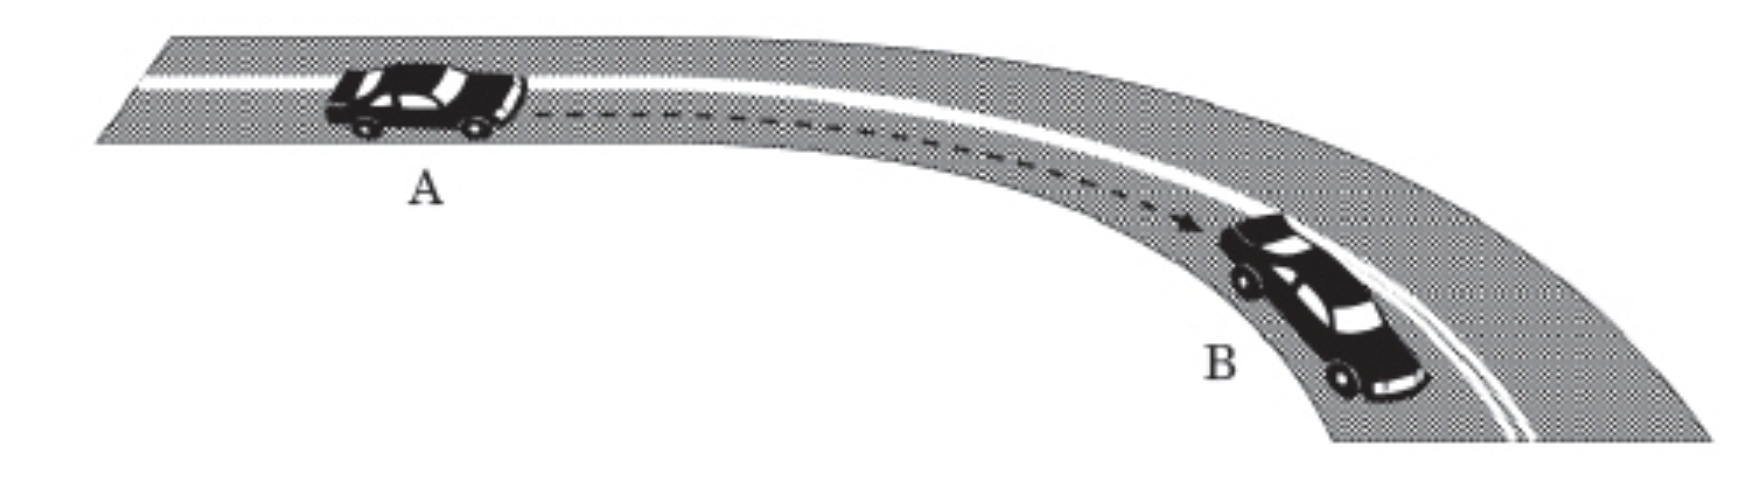
\includegraphics[width=6cm]{physics/figures/figure-unit-3-car-curve.png}
\end{center}

Which of the following describes the car’s acceleration?
\clearpage

\begin{randomizechoices}[keeplast]
    \correctchoice The car is accelerating because it changes direction.
    \choice The car is accelerating because it moves at constant speed.
    \choice The car is not accelerating because it went away from the reference point.
    \choice none of the above
\end{randomizechoices}

\question 
Which of the following pair of graphs demonstrates an object moving away from the reference point with a decreasing velocity?

\bigskip

\begin{minipage}{0.45\textwidth}
\centering
\textbf{Pair A}

\vspace{1ex}

\begin{tikzpicture}
    \begin{axis}[height=4cm,
        width=4cm,
        ymin=0,ymax=5,
        xmin=0,xmax=3,
        ticks=none,
        axis lines=left,
        ylabel={$x$},
        y label style={rotate=-90},
        xlabel={$t$},
    ]
        \addplot[domain=0:2,very thick,black] {(x-2)^2};
    \end{axis}
\end{tikzpicture}
\begin{tikzpicture}
    \begin{axis}[height=4cm,
        width=4cm,
        ymin=-3,ymax=3,
        xmin=0,xmax=3,
        ticks=none,
        axis y line=left,
        axis x line=center,
        ylabel={$v$},
        y label style={rotate=-90},
        xlabel={$t$},
        clip=false
    ]
        \addplot[domain=0:2.5,very thick,black] {-x};
        \draw (0,-3) node[below,white] {$t$}; %...FOR ALIGNMNET
    \end{axis}
\end{tikzpicture}
\end{minipage}%
\begin{minipage}{0.45\textwidth}
\centering
\textbf{Pair B}

\vspace{1ex}

\begin{tikzpicture}
    \begin{axis}[height=4cm,
        width=4cm,
        ymin=0,ymax=5,
        xmin=0,xmax=3,
        ticks=none,
        axis lines=left,
        ylabel={$x$},
        y label style={rotate=-90},
        xlabel={$t$},
    ]
        \addplot[domain=0:2,very thick,black] {4*x - x^2};
    \end{axis}
\end{tikzpicture}
\begin{tikzpicture}
    \begin{axis}[height=4cm,
        width=4cm,
        ymin=-3,ymax=3,
        xmin=0,xmax=3,
        ticks=none,
        axis y line=left,
        axis x line=center,
        ylabel={$v$},
        y label style={rotate=-90},
        xlabel={$t$},
        clip=false
    ]
        \addplot[domain=0:2.5,very thick,black] {-x+2.5};
        \draw (0,-3) node[below,white] {$t$}; %...FOR ALIGNMNET
    \end{axis}
\end{tikzpicture}
\end{minipage}

\vspace{1em}

\begin{minipage}{0.45\textwidth}
\centering
\textbf{Pair C}

\vspace{1ex}

\begin{tikzpicture}
    \begin{axis}[height=4cm,
        width=4cm,
        ymin=0,ymax=5,
        xmin=0,xmax=3,
        ticks=none,
        axis lines=left,
        ylabel={$x$},
        y label style={rotate=-90},
        xlabel={$t$},
    ]
        \addplot[domain=0:2,very thick,black] {4*x-x^2};
    \end{axis}
\end{tikzpicture}
\begin{tikzpicture}
    \begin{axis}[height=4cm,
        width=4cm,
        ymin=-3,ymax=3,
        xmin=0,xmax=3,
        ticks=none,
        axis y line=left,
        axis x line=center,
        ylabel={$v$},
        y label style={rotate=-90},
        xlabel={$t$},
        clip=false
    ]
        \addplot[domain=0:2.5,very thick,black] {-x};
        \draw (0,-3) node[below,white] {$t$}; %...FOR ALIGNMNET
    \end{axis}
\end{tikzpicture}
\end{minipage}%
\begin{minipage}{0.45\textwidth}
\centering
\textbf{Pair D}

\vspace{1ex}

\begin{tikzpicture}
    \begin{axis}[height=4cm,
        width=4cm,
        ymin=0,ymax=5,
        xmin=0,xmax=3,
        ticks=none,
        axis lines=left,
        ylabel={$x$},
        y label style={rotate=-90},
        xlabel={$t$},
    ]
        \addplot[domain=0:2,very thick,black] {(x-2)^2};
    \end{axis}
\end{tikzpicture}
\begin{tikzpicture}
    \begin{axis}[height=4cm,
        width=4cm,
        ymin=-3,ymax=3,
        xmin=0,xmax=3,
        ticks=none,
        axis y line=left,
        axis x line=center,
        ylabel={$v$},
        y label style={rotate=-90},
        xlabel={$t$},
        clip=false
    ]
        \addplot[domain=0:2.5,very thick,black] {-x+2.5};
        \draw (0,-3) node[below,white] {$t$}; %...FOR ALIGNMNET
    \end{axis}
\end{tikzpicture}
\end{minipage}


{\color{white}
\begin{randomizeoneparchoices}[norandomize,]
    \choice Pair A
    \correctchoice Pair B
    \choice Pair C
    \choice Pair D
\end{randomizeoneparchoices}
}




\question
What is happening in this graph?

\begin{center}
    \begin{tikzpicture}
        \begin{axis}[width=4cm,
            height=4cm,
            axis y line=left,
            axis x line=center,
            ymin=-2,ymax=2,
            xmin=0,xmax=2,
            ytick={-2,-1,...,2},
            xtick=\empty,
            ylabel={Velocity},
            xlabel={$t$},
            ]
            \draw[very thick] (0,0) -- (1.8,-1.8);
        \end{axis}
    \end{tikzpicture}%
    \hspace{1cm}
    \begin{tikzpicture}[scale=0.8,rotate=10,transform shape]
            \draw (0,0) rectangle ++(10,-0.5) node[pos=0.12,below=-2pt] {0 position} node[pos=0.98,above] {$+$};
            \draw[above=9mm] (8,0) rectangle ++(1.5,-0.7) node[pos=0.5,below=-3mm] {cart};
            \draw[fill=white,above=2mm] (8.4,0) circle (2mm);
            \draw[fill=white,above=2mm] (9.1,0) circle (2mm);
            \draw[above=0.5cm,ultra thick,->] (8,0) -- ++(-1.5,0);
    \end{tikzpicture}
\end{center}

\begin{randomizechoices}
    \choice negative velocity, positive acceleration, increasing speed
    \choice positive velocity, positive acceleration, increasing speed
    \choice negative velocity, negative acceleration, decreasing speed
    \correctchoice negative velocity, negative acceleration, increasing speed
\end{randomizechoices}

\question
A runner moves according to the velocity vs time graph shown below. What is the acceleration of the runner at 3 seconds?

\begin{minipage}{0.3\textwidth}
    \centering
\begin{randomizechoices}
    \choice \SI{12}{m/s^2}
    \choice \SI{2}{m/s^2}
    \correctchoice \SI{3}{m/s^2}
    \choice \SI{6}{m/s^2}
\end{randomizechoices}
\end{minipage}%
\hspace{1em}
\begin{minipage}{0.45\textwidth}
\centering
    \begin{tikzpicture}
        \begin{axis}[height=5cm,
            width=7cm,
            ylabel={Velocity (m/s)},
            xlabel={Time (s)},
            ymin=0,ymax=14,
            xmin=0,xmax=12,
            ytick={0,2,...,14},
            xtick={0,2,...,12},
            axis lines=left,
            grid=both,
            % title={Runner Velocity vs. Time}
        ]
        \addplot[very thick,black] coordinates{(0,0)(4,12)(6,12)(8,12)(10,12)(12,6)};
        \end{axis}
    \end{tikzpicture}
\end{minipage}



% \question
% The rate at which an object’s velocity changes is called its \fillin[acceleration].


\clearpage

\thispagestyle{headandfoot}
\header{Physics\\Test on Unit 3: Changing Motion}{}{{Name:\enspace\makebox[5cm]{\hrulefill}}}



\question[2]
The following shows a velocity vs. time graph, and a student's INCORRECT calculation of the object's average acceleration using two data points.

\begin{minipage}{0.45\textwidth}
\begin{tikzpicture}
\begin{axis}[width=7cm,height=6cm,
    axis lines=left,
    % axis x line=center,
    xlabel = {Time (s)},
    ylabel = {Velocity (m/s)},
    ymin=0, ymax=14,
    xmin=0, xmax=10,
    ytick={0,2,...,14},
    xtick={0,1,...,10},
    ymajorgrids=true,
    xmajorgrids=true,
]
    \addplot[very thick,black,domain=0:10] {-3/2*\x+18};
    \fill (4,12) circle (2pt);
    \fill (8,6) circle (2pt);
    \end{axis}
\end{tikzpicture}
\end{minipage}%
\begin{minipage}{0.45\textwidth}
\begin{align*}
    a = \frac{\Delta v}{\Delta t} &= \frac{v_f - v_i}{t_f - t_i} \\[1ex]
    &=  \frac{8 - 4}{6 - 12} \\[1ex] 
    &= \boxed{\SI{-0.67}{m/s^2}}
\end{align*}
\end{minipage}

Explain why the student's calculation is wrong. Then calculate the actual acceleration of the object.

\begin{solutionorbox}[6cm]
\phantom{.}

\textbf{1 point earned}: For identifying that the numbers were plugged into the fraction incorrectly or for indicating that the fraction should be flipped.

In the numerator, the student calculated change in time, and they calculated change in velocity in the denominator. Therefore, since acceleration is change in velocity vs. change in time, the fraction should be flipped.

\textbf{1 point earned}: For correctly computing average acceleration:

\begin{align*}
    a = \frac{\Delta v}{\Delta t} &= \frac{v_f - v_i}{t_f - t_i} \\[1ex]
    &=  \frac{6 - 12}{8 - 4} \\[1ex] 
    &= \boxed{\SI{-1.5}{m/s^2}}
\end{align*}

or $a = -\frac{3}{2} \mathrm{m/s^2}$.
\end{solutionorbox}

\question[2]
If an 80\,kg cannonball accelerates from rest to \SI{28}{m/s} in 2 seconds, what is the net force on the cannonball?

\begin{solutionorbox}[6cm]
\phantom{.}

\textbf{1 point earned}: For computing acceleration:

\begin{equation*}
    a = \frac{\Delta v}{\Delta t} = \SI{14}{m/s^2}
\end{equation*}

\textbf{1 point earned}: For computing net force:

\begin{equation*}
    F_\mathrm{net} = ma = (\SI{80}{kg})(\SI{14}{m/s^2}) = \boxed{\SI{1120}{N}}
\end{equation*}
\end{solutionorbox}

\clearpage

\header{Physics}{}{Unit 3 Test}

\question [2]
Consider the table below.

\begin{center}
    \begin{tabular}{|c|c|c|}
        \hline
        \textbf{Time} (s) & \textbf{Speed} (m/s) & \textbf{Direction} \\ \hline
        8 & 16 & East\\ \hline
        9 & 20 & East\\ \hline
        10 & 24 & East\\ \hline
        11 & 28 & East\\ \hline
    \end{tabular}
\end{center}

Does this table represent an object that is accelerating? How do you know? Explain.

\fillwithlines{3cm}

\begin{solutionorbox}
\phantom{.}

\textbf{1 point earned}: For stating that the object's velocity is increasing with time.

\textbf{1 point earned}: For stating that acceleration is the rate of change in velocity, so that a change in velocity implies acceleration.
\end{solutionorbox}

\question [2]
A cart moves on a straight track and its motion is recorded in the graph below.

\begin{center}
\begin{tikzpicture}
    \begin{axis}[height=6cm,
        width=6cm,
        ymin=0,ymax=5,
        xmin=0,xmax=3,
        ticks=none,
        axis lines=left,
        ylabel={$x$},
        y label style={rotate=-90},
        xlabel={$t$},
    ]
        \addplot[domain=0:2,very thick,black] {4*(x+2) - (x+2)^2};
        \fill ({0.4},{4*(0.4+2) - (0.4+2)^2}) circle (2pt) node[above=2pt] {A};
        \fill ({1.2},{4*(1.2+2) - (1.2+2)^2}) circle (2pt) node[above right] {B};
        \fill ({1.8},{4*(1.8+2) - (1.8+2)^2}) circle (2pt) node[above right] {C};
    \end{axis}
\end{tikzpicture}
\end{center}

Points A, B, and C represent three different instants in time. Rank these points according to the object's speed at those instants, from the fastest point to the slowest.

\begin{solutionorbox}[6cm]
\phantom{.}

\textbf{1 point earned}: For ranking the points from fastest to slowest speed of the object as C, B, A. 

\textbf{1 point earned}: For explaining that the steepness or slope of the curve at the points indicates the object's velocity; the object undergoes bigger changes in position for a small interval of time centered at C than it does for an equal interval of time centered at A.
\end{solutionorbox}

\ifprintanswers
\clearpage

{\large
\printkeytable
}
\fi
\end{questions}
\end{document}

